\section{Предсказание волатильности}
После реализации биржи можно, наконец, перейти к исследованию по предсказанию динамики торговой нагрузки на нее.

Прежде всего необходимо формализовать само понятие "биржевая нагрузка", чтобы понять какую величину мы хотим предсказывать. В рамках этой работы мы сделаем это следующим образом:

\begin{quote}
\textbf{Биржевая нагрузка} - количество входящих заявок, поступающих за одну секунду.
\end{quote}

От ее величины будет зависеть заполненность буффера, о которой было упомянуто в пункте про нагрузочное тестирование.


\subsection{Данные}

Для анализа и обучения были выбраны данные торгов криптовалюты Bitcoin.
Криптовалюты более всего удобны для исследований, прежде всего потому что эта сфера финансов одна из самых открытых и доступных: 
торговую историю можно без дополнительных вложений получить практически от любой криптовалютной биржи. Кроме того, эти данные имеют удобный формат: биржевые стаканы имеют достаточную глубину в 10-20 котировок, а временные моменты расписаны с точностью до миллисекунд.



\subsection{Предсказывающие модели}


Ниже приведены наложенные графики двух величин: ценa и количество запров за некоторый промежуток времени.

\begin{center}
    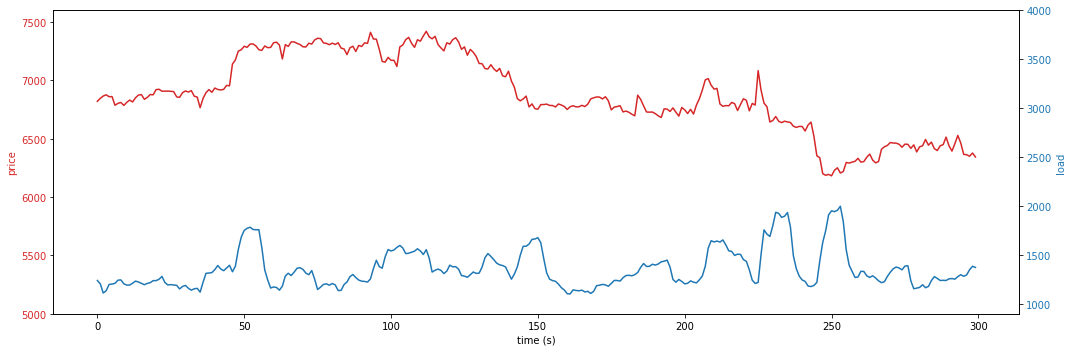
\includegraphics[width=450pt]{images/graph_price_load.png}
\end{center}

Можно видеть, что количество запросов коррелирует с динамикой цены: после резких скачков цены происходит также резкое повышение количества запросов, обусловленное стремлением рынка к корректировке. Это вполне очевидная зависимость, поэтому мы действительно можем подразумевать под волатильностью как скорость изменения цены, так и величину биржевой нагрузки.

\newpage

Посмотрим также на график наполненности буффера запросов, наложенный на график количества запросов:
\begin{center}
    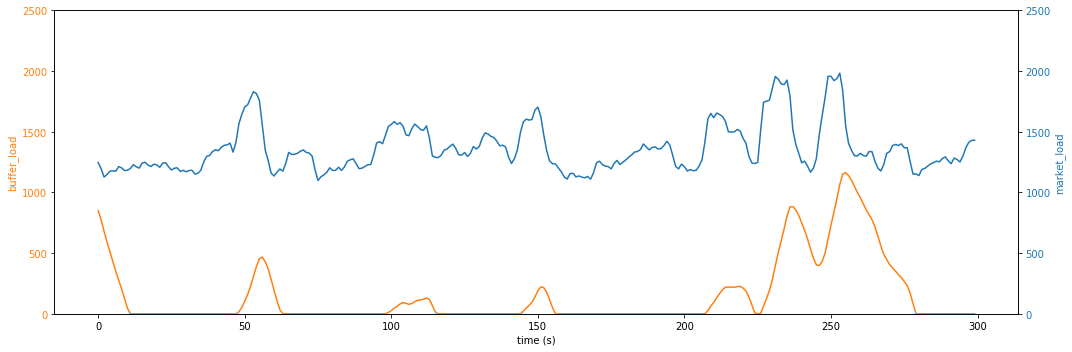
\includegraphics[width=450pt]{images/graph_buffer_load.png}
\end{center}

Видно, что при достижении количества запросов от клиентов некоторого порогового значения около 1500 запросов в секунду, наполненность буффера начинает расти из-за того, что торговый движок не успевает обрабатывать заявки.

\subsubsection{Статистическая модель}

По графикам выше можно предположить, что для предсказания нагрузки достаточно использовать простую статистическую модель, основанную, например, на скользящем среднем.

И действительно, поскольку резкое изменение цены является надежным сигналом к последующей реакции рынка, мы можем отслеживать ценовую динамику за последние секунды
и на основании этого делать прогнозы по увеличению количества поступающих запросов.

Для этого будем использовать модель из пакета

\textbf{statsmodels.tsa.arima\_model} под названием \textbf{ARMA}, являющуюся обобщением авторегрессии и скользащего среднего [2.1], [2.2].

Предсказание будет производиться в два этапа:
\begin{itemize}
    \item 1. Преобразуем временной ряд цен во временной ряд разниц цен
    \item 2. По временному ряду разниц цен будем предсказывать биржевую нагрузку с помощью ARMA
\end{itemize}

Полученный временной ряд с разницами цен, наложенный на график нагруженности:

\begin{center}
    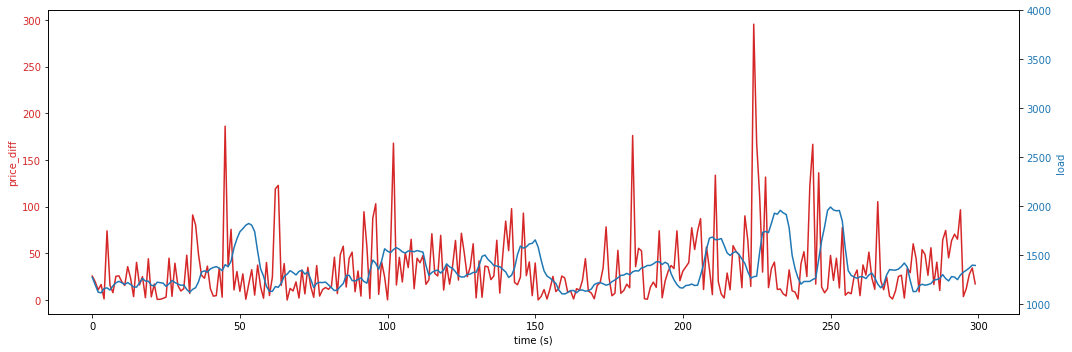
\includegraphics[width=450pt]{images/graph_diff_load.png}
\end{center}

Видно, что повышению нагрузки предшествуют резкие скачки цены. Для удобства можно оставить только те значения разниц цен, которые больше некоторого порогового значения:


\begin{center}
    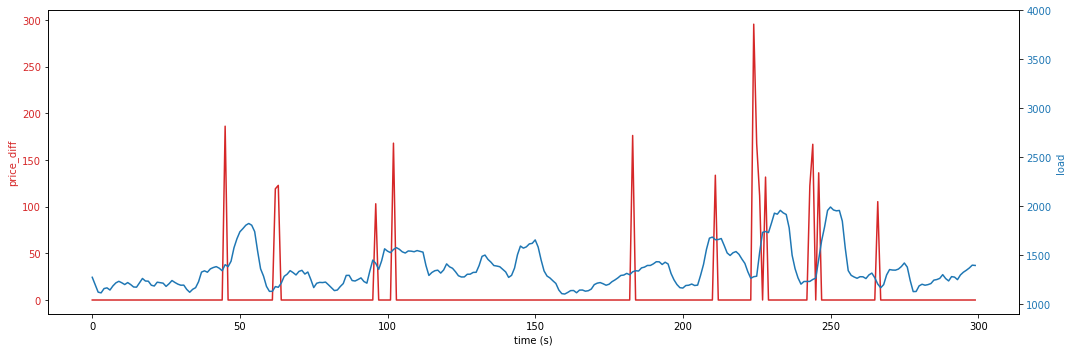
\includegraphics[width=450pt]{images/graph_diff_load_2.png}
\end{center}

Попробуем теперь предсказывать разницу цен с помощью ARMA. График такого предсказания:


\begin{center}
    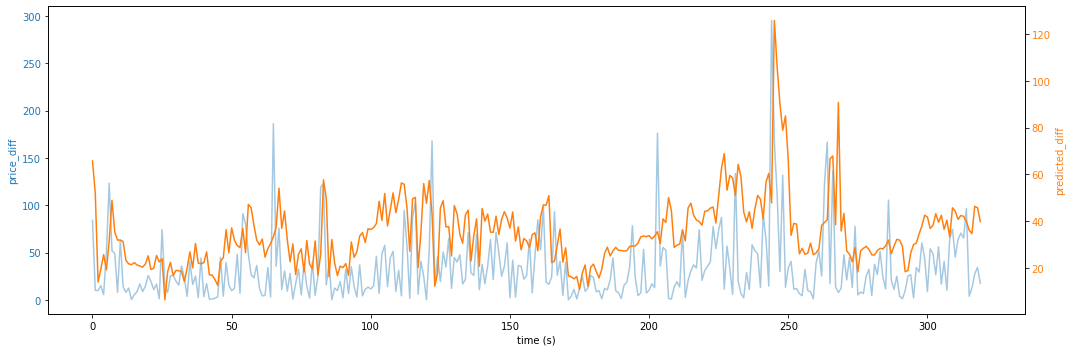
\includegraphics[width=450pt]{images/graph_arma_prediction.png}
\end{center}

Видно, что на больших пиках (в районе 200 сек) предсказание довольно успешно. Однако средние повышения остаются не предсказанными.
\newpage
\subsubsection{Рекуррентные сети}

Одними из самых распространенных моделей для предсказания временных рядов в финансах традиционно считаются рекуррентные сети. Вкратце разберем, как они работают [2.3], [2.4].

Обычная нейронная сеть состоит из набора слоев с нейронами, последовательно соединенными друг с другом. На вход поступает некоторый набор значений, он проходит через все слои и на выходе выдается некоторая величина в качестве ответа.


\begin{center}
    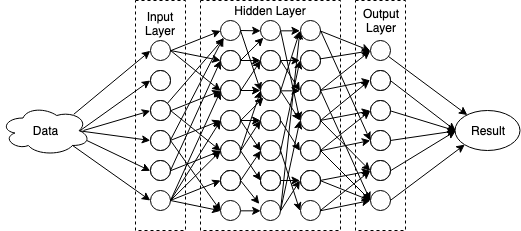
\includegraphics[width=450pt]{images/network_schema.png}
\end{center}

В рекуррентной же сети добавляется еще одно входное значение - предсказание модели на предыдущем шаге:

\begin{center}
    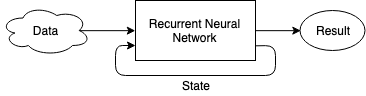
\includegraphics[width=300pt]{images/network_schema_2.png}
\end{center}
\newpage

Это можно для удобства раскрыть как несколько сетей, каждая из которых передает значение предсказания в следующую:

\begin{center}
    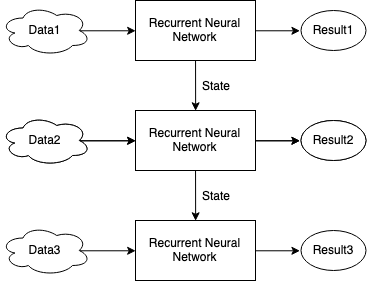
\includegraphics[width=300pt]{images/network_schema_3.png}
\end{center}

Такая архитектура позволяет хранить некоторый контекст, в котором происходит предсказание. На практие это это дает значительное улучшение в результатах, и используется, например, в предсказании погоды [2.5].
\newpage
Я использовал простую реализацию \textbf{RNN} из пакета \textbf{keras}.

Ниже приведена полная конфигурация сети:
\begin{small}
\begin{verbatim}
    Model: "sequential_3"
______________________________________________
Layer (type)    Output Shape   Param #   
==============================================
simple_rnn_3 (SimpleRNN) (None, 32)        1184      
______________________________________________
dense_5 (Dense)          (None, 8)         264       
______________________________________________
dense_6 (Dense)          (None, 1)         9         
==============================================
Total params: 1,457
Trainable params: 1,457
Non-trainable params: 0
______________________________________________
\end{verbatim}
\end{small}

Полученные в результате работы предсказания:

\begin{center}
    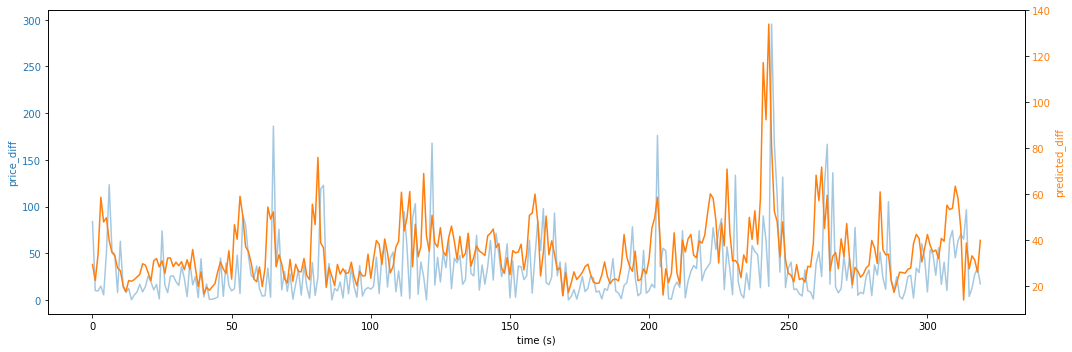
\includegraphics[width=450pt]{images/graph_rnn_prediction.png}
\end{center}

Видно, что предсказания стали точнее: пики изменения цен, предшествующие повышению нагрузки, стали отчетливее и соответствуют тому, что происходило в реальности.
\newpage

\subsection{Сравнительное тестирование}

В качестве критерия качества предсказаний полученных моделей я выбрал способность давать правильные сигналы-предупреждения о надвигающейся активности.

Для этого на исходных данных я разметил моменты, когда поступающие запросы превосходят производительность торгового движка (1500 запросов в секунду).

Корректным сигналом считается превышение порогового значения $P$ в предсказании от модели. Я провел несколько экспериментов с различными константами, результаты F-меры приведены в таблице ниже.


\begin{center}
\begin{tabular}{ c c c }
 P & ARMA & RNN \\ 
40 & 0.60 & 0.84 \\
50 & 0.71 & 0.97 \\
60 & 0.54 & 0.98 \\
70 & 0.54 & 0.77 \\
80 & 0.54 & 0.66 \\
90 & 0.54 & 0.60 \\
\end{tabular}
\end{center}

Таким образом, наилучшие значения предсказания достигаются при $P = 50$.

\newpage